\chapter{A convolutional neural network for CHIPS}
\label{chap:cvn}

Here are some funky floats using ``continued captions'', i.e. for a semantically
collected group of float contents which are too numerous to fit into a single
float, such as the pretty circles in the following figure

\section{Convolutional Neural Networks}
\label{sec:cnn}

\section{CHIPS Events}
\label{sec:events}

\begin{figure}
    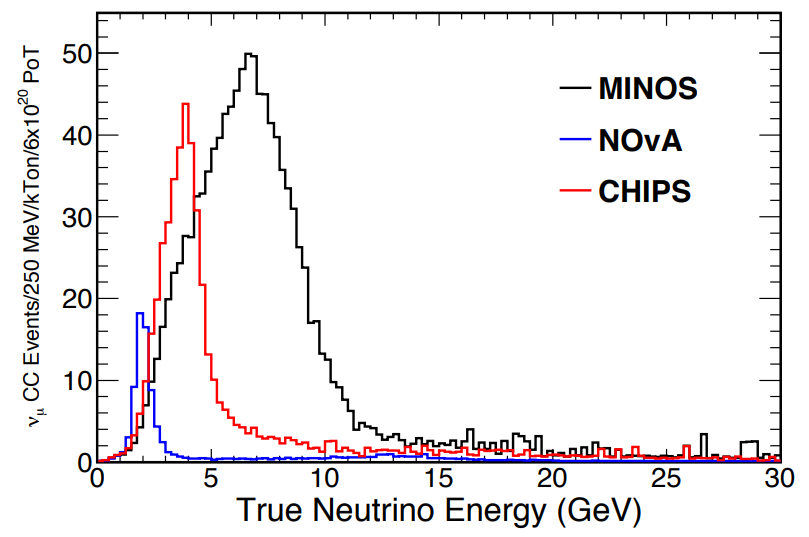
\includegraphics[width=\largefigwidth]{diagrams/numi_axis}
    \caption[CKM Fitter constraints on \alphaCKM.]%
    {CKM Fitter constraints on \alphaCKM from combined \BToPiPi,
        \BToRhoPi and \BToRhoRho decay analyses.}
    \label{fig:numi_axis}
\end{figure}

\begin{figure}
    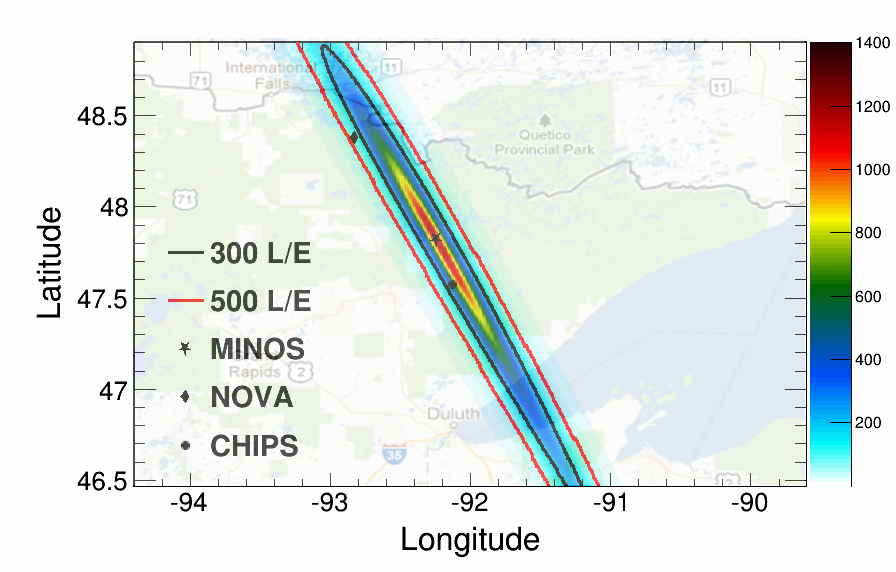
\includegraphics[width=\largefigwidth]{diagrams/numi_map}
    \caption[CKM Fitter constraints on \alphaCKM.]%
    {CKM Fitter constraints on \alphaCKM from combined \BToPiPi,
        \BToRhoPi and \BToRhoRho decay analyses.}
    \label{fig:numi_map}
\end{figure}

The expected beam flux at the CHIPS detector location is found from reweighting current

We can use current NuMI beam simulations

Current NuMI beam experiments

